\chapter{Implementação computacional}

A implementação computacional do programa foi feita com base na linguagem livre Python, utilizando as vantagens e facilidades que os pacotes dela provém.  
O algoritmo deste trabalho será distribuído livremente sob a licença BSD 3-clause como parte do \textit{Fatiando a Terra} \citet{uieda-proc-scipy-2013}, que é uma biblioteca Python livre, usada para modelagem e inversão em geofísica. As documentações e instruções para instalação da versão mais atual do \textit{Fatiando a Terra} podem ser encontrados em http://www.fatiando.org.
Os códigos e documentações sobre instalação e uso do programa podem ser encontrados no Github pelo link: https://github.com/DiegoTaka/ellipsoid-magnetic
O uso do programa é bastante facilitado e consiste em apenas colocar os parâmetros necessários para gerar o corpo elipsoidal como mostra a Figura \ref{fig:Cookbook_Triaxial}.

Como mostrado neste exemplo, é necessário importar outras ferramentas do próprio \textit{Fatiando a Terra} antes de criar o modelo elipsoidal desejado.

\begin{figure}[hbt!]
	\centering 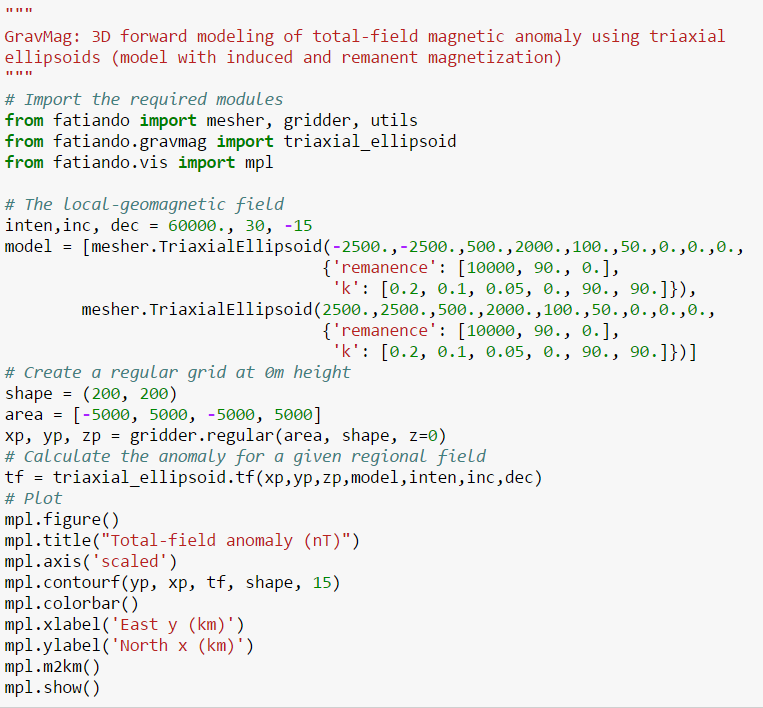
\includegraphics[width=16 cm,height=16 cm]{figures/Cookbook_Triaxial}
	\caption[Cookbook para gerar um modelo elipsoidal triaxial e calcular a anomalia de campo total.]{Cookbook para gerar um modelo elipsoidal triaxial e calcular a anomalia de campo total aproximada.}
	\label{fig:Cookbook_Triaxial}
\end{figure}

Em \textit{''The regional field''} é necessário colocar o campo regional (intensidade ($nT$), inclinação e declinação $(º)$).

Em \textit{''bounds''} o tamanho do \textit{grid} onde será feito os cálculos.

Em \textit{''model''} é criado o modelo através da classe \textit{''ellipsoid triaxial''}. Os parâmetros são, respectivamente: posição $x$, $y$ e $z$ ($m$) do centro do corpo, semi-eixos $a$, $b$ e $c$ ($m$), orientações de $azimute$, $\beta$ e $\gamma$ $(º)$. 
Dentro do dicionário \textit{'remanence'} a intensidade ($A/m$), inclinação e declinação $(º)$ do vetor de magnetização remanente. Já dentro do dicionário \textit{'k'} os valores de $k1$, $k2$ e $k3$ de susceptibilidade (SI) e as orientações de azimute, inclinação $(º)$ e \textit{tilt} que formam os vetores de susceptibilidade.
Em  \textit{''shape''} é dado quantos pontos serão calculados dentro da área escolhida na malha criada em $xp$, $yp$ e $zp$.
Em \textit{''tf''} é calculado a anomalia de campo total aproximada dados os parâmetros e modelo elipsoidal criado.
Abaixo é dado a \textit{plotagem} da figura.

As classes elipsoidais criadas no \textit{''mesher''} são separadas para cada um dos casos de elipsoide. Neles são guardados os parâmetros geométricos do objeto e suas propriedades físicas. A classe elipsoidal também inclui a função para o cálculo da matriz de transformação de coordenadas. Na documentação também são inclusos testes automáticos para verificar a integridade das classes e funções. Já na biblioteca \textit{''gravmag''} é onde se encontra as funções que de fato calculam o campo magnético e a anomalia total aproximada como exemplificada na Figura \ref{fig:func_triaxial}, do modelo criado no \textit{''mesher''}.
\begin{figure}[hbt!]
	\centering 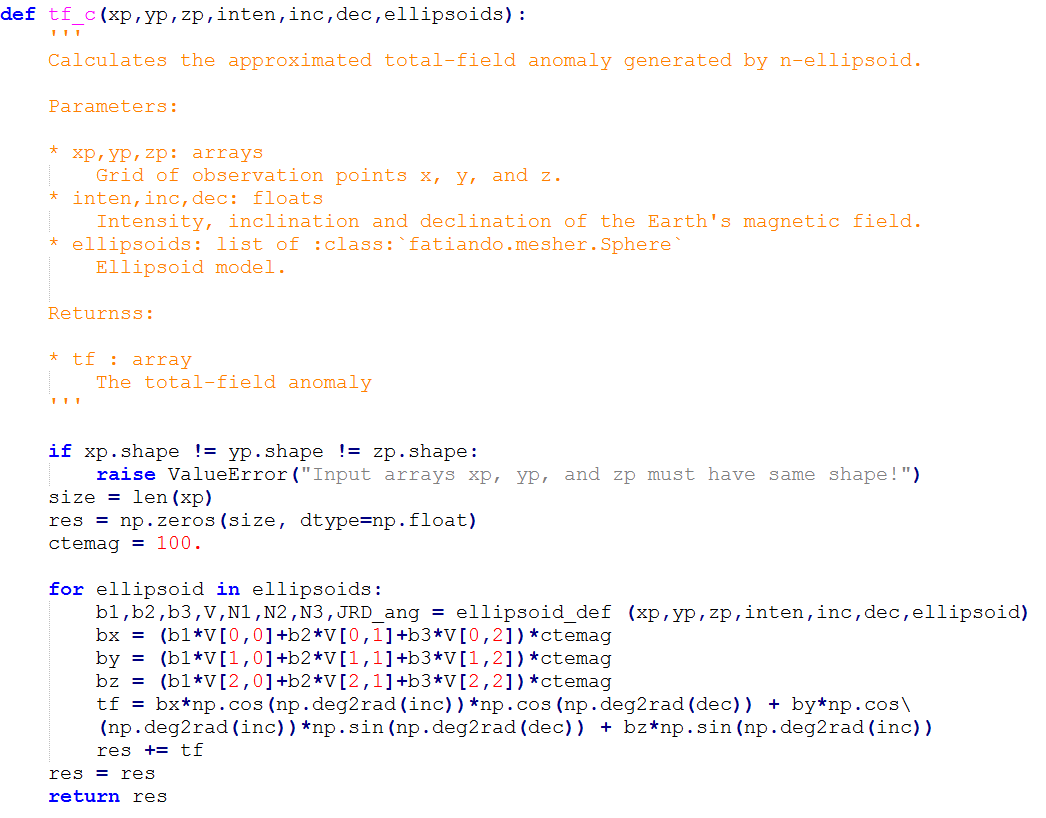
\includegraphics[width=16 cm,height=16 cm]{figures/func_triaxial}
	\caption[Função que calcula a anomalia de campo total aproximada de um elipsoide triaxial.]{Função que calcula a anomalia de campo total aproximada de um elipsoide triaxial.}
	\label{fig:func_triaxial}
\end{figure}

Os cálculos de $b1$, $b2$, $b3$ e $V$ estão descritos na seção de metodologia deste trabalho.

É importante ressaltar que diversos cálculos são feitos com auxílio de bibliotecas do \textit{Python} como o \textit{Scipy} \citet{scipy}, \textit{Matplotlib} \citet{matplotlib} e do pacote \textit{NumPy} \citet{numpy}.

Uma nota a respeito das funções \textit{scipy.special.ellipkinc} e \textit{scipy.special.ellipeinc} do pacote SciPy para o cálculo das integrais elípticas normais incompletas de Legendre de primeiro e segundo tipo: a variável $k$ das funções $F(\kappa, \phi)$ e $E(\kappa, \phi)$ já deve ser elevada ao quadrado quando utilizada como argumento, uma vez que, no pacote Scipy, sua implementação não é feita com a fórmula comumente encontrada, onde geralmente se usa $k^2$:
\begin{equation}
F(\kappa, \phi) = \int_{0}^{\phi}{\dfrac{d\theta}{\sqrt{1-k^{2}sin^{2}\theta}}} \quad 0\le\theta\le\pi/2
\label{eq:integral_elip1}
\end{equation}
e
\begin{equation}
E(\kappa, \phi) = \int_{0}^{\phi}{\sqrt{1-k^{2}sin^{2}\theta}} \quad d\theta
\label{eq:integral_elip2}
\end{equation}

Uma forme eficiente de testar se essas integrais estão corretas é verificar se a soma dos fatores de desmagnetização é igual à 1 (um), independente do tamanho dos eixos do elipsoide, como mostra a Figura \ref{fig:teste_n_soma}
\begin{figure}[hbt!]
	\centering 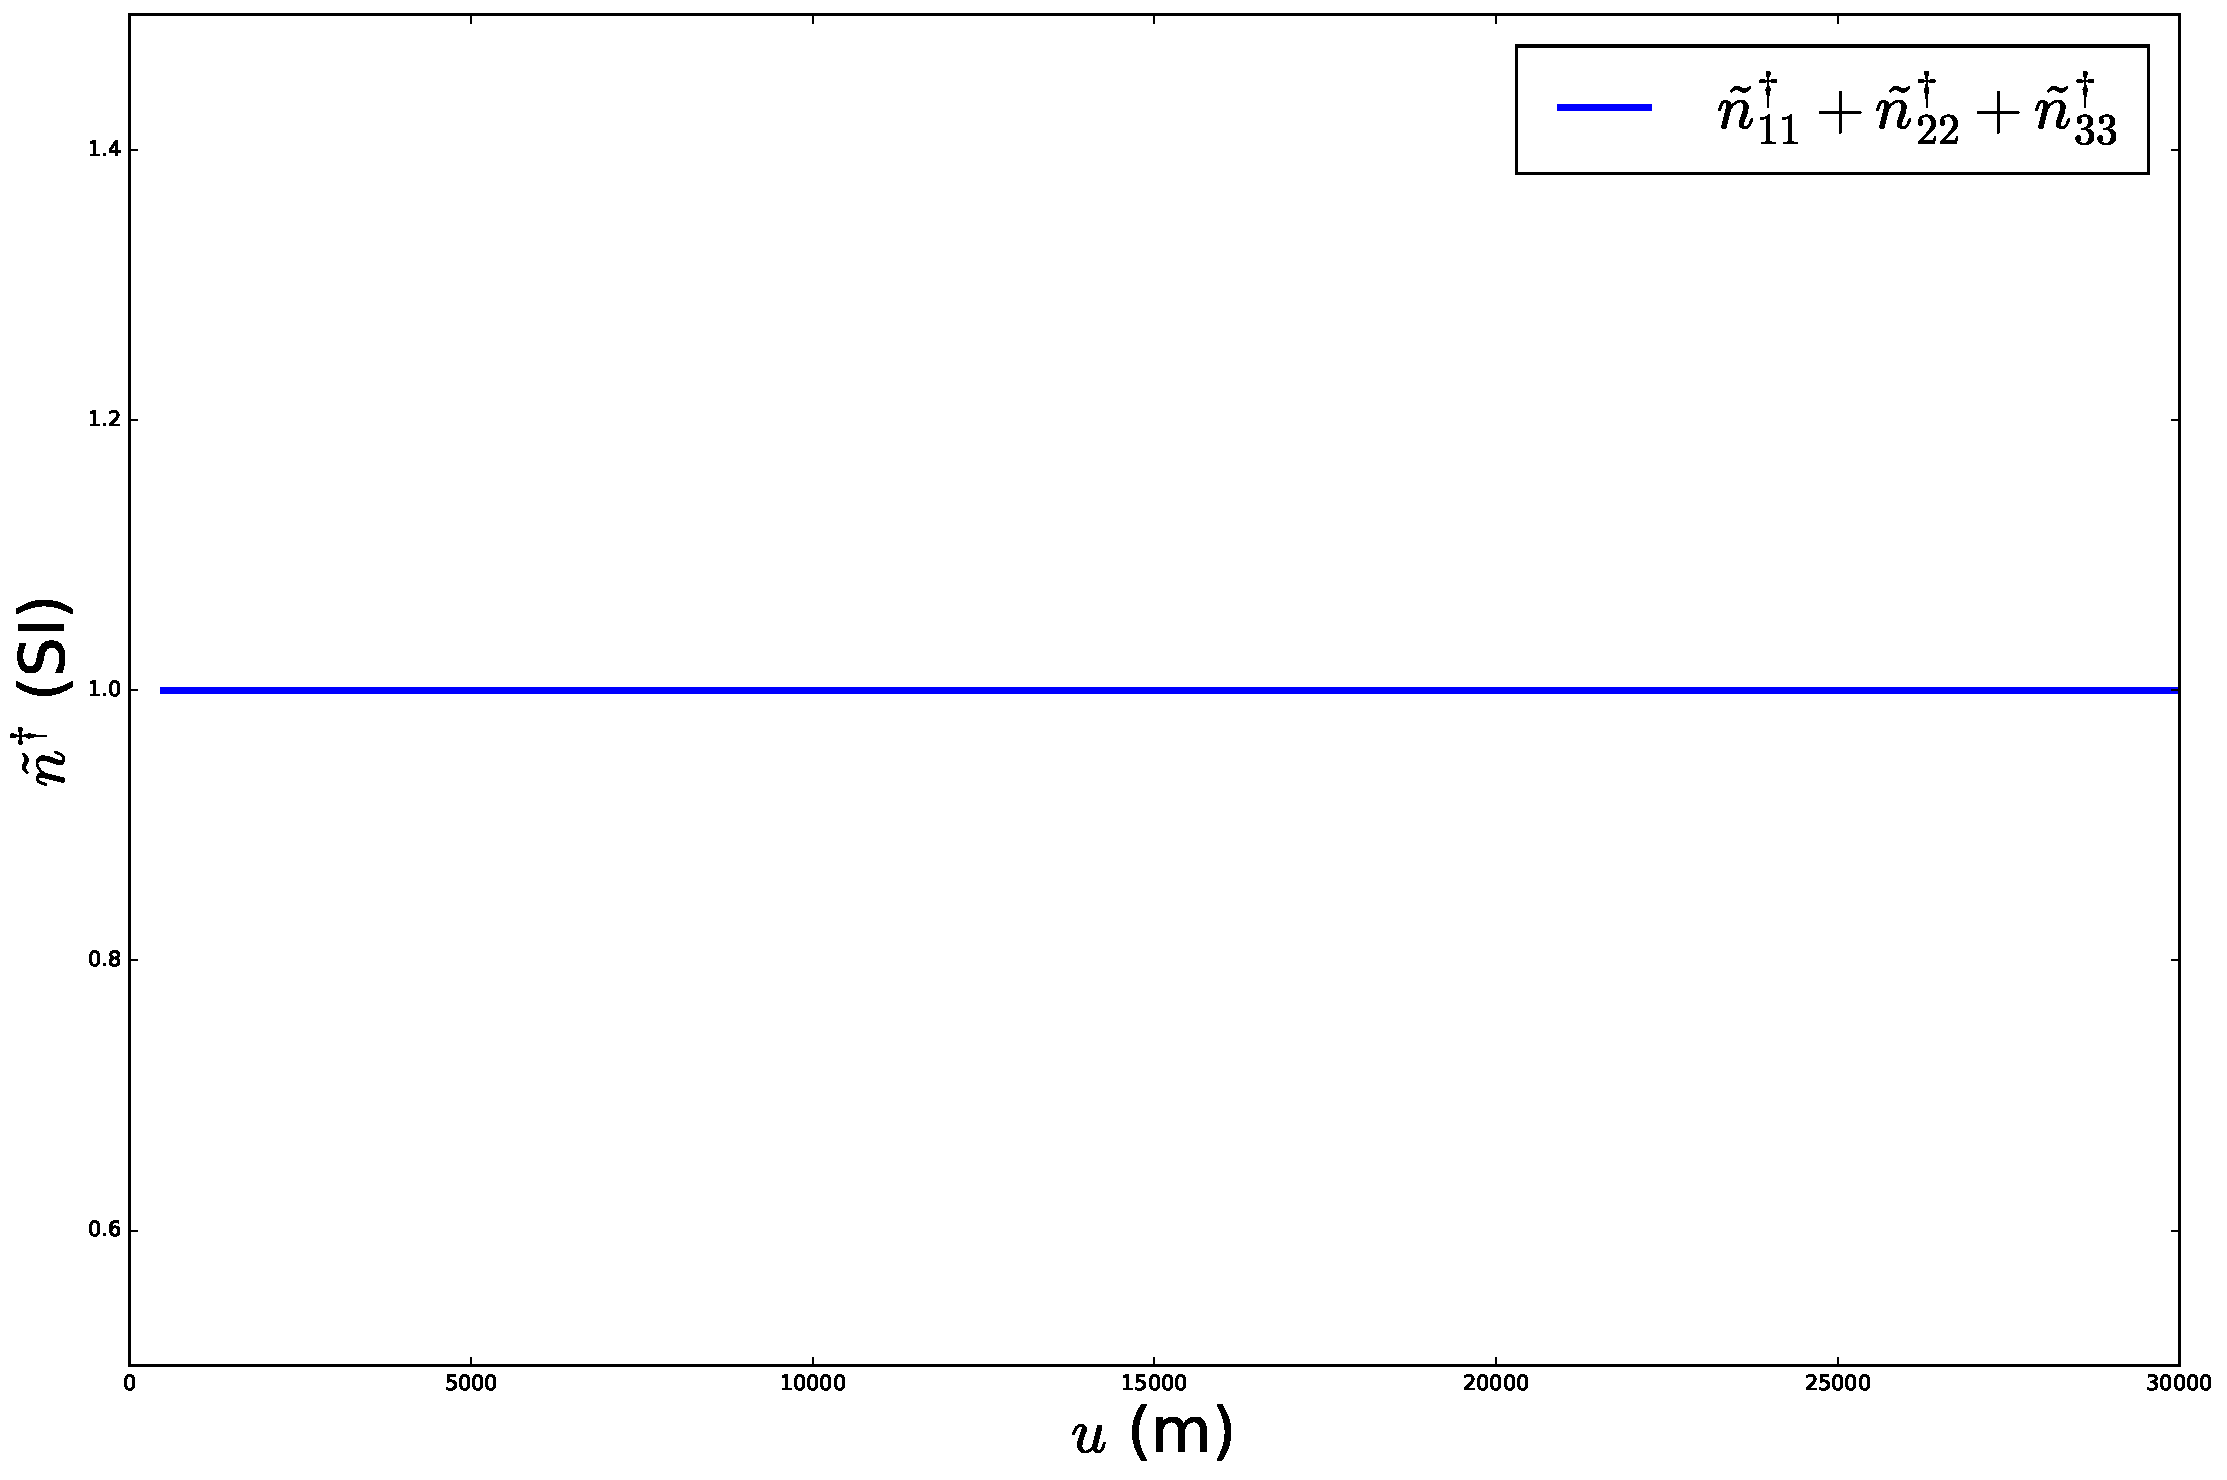
\includegraphics[width=15 cm,height=10 cm]{figures/test_n_soma}
	\caption[Soma dos fatores de desmagnetização. No SI a soma deverá ser igual à 1 (um).]{Soma dos fatores de desmagnetização. No SI a soma deverá ser igual à 1 (um). O fator $u$ são números reais crescentes, que soma, simultaneamente, todos os semi-eixos.}
	\label{fig:teste_n_soma}
\end{figure}
